% Cluster Kit project report.  Build:  tectonic -X compile report.tex
\documentclass[11pt,a4paper]{article}
\usepackage[a4paper,margin=2.5cm]{geometry}
\usepackage{fontspec}
\setmainfont{texgyrepagella}[Extension=.otf,UprightFont=*-regular,BoldFont=*-bold,ItalicFont=*-italic,BoldItalicFont=*-bolditalic]
\usepackage{graphicx,booktabs,tabularx,array,float,csquotes,caption,needspace,enumitem,eso-pic}
\usepackage{xcolor,titlesec,colortbl}
\usepackage{tikz,pgfplots}
\definecolor{hblue}{HTML}{7B1E2B}
\definecolor{accent}{HTML}{C0504D}
\definecolor{gblue}{HTML}{1F3A5F}
\titleformat*{\section}{\Large\bfseries\color{hblue}}
\titleformat*{\subsection}{\large\bfseries\color{hblue}}
\renewcommand{\abstractname}{\color{hblue}Abstract}
\pgfplotsset{compat=1.18}
\usetikzlibrary{arrows.meta,positioning}
\usepackage[hidelinks]{hyperref}

\captionsetup{font=small,labelfont={bf,color=hblue}}
\setlength{\parindent}{0pt}
\setlength{\parskip}{6pt}
\usepackage{microtype}
\setlist{itemsep=1pt,topsep=2pt}
\newcolumntype{L}{>{\raggedright\arraybackslash}X}
% keep a heading on the same page as what follows it
\let\oldsection\section
\renewcommand{\section}{\Needspace{6\baselineskip}\oldsection}
\let\oldsubsection\subsection
\renewcommand{\subsection}{\Needspace{5\baselineskip}\oldsubsection}

% double-line border on every page
\AddToShipoutPictureBG{\AtPageLowerLeft{\begin{tikzpicture}
  \useasboundingbox (0,0) rectangle (\paperwidth,\paperheight);
  \draw[black,line width=1.2pt] (1.2cm,1.2cm) rectangle (\paperwidth-1.2cm,\paperheight-1.2cm);
  \draw[black,line width=0.4pt] (1.38cm,1.38cm) rectangle (\paperwidth-1.38cm,\paperheight-1.38cm);
\end{tikzpicture}}}

\tikzset{box/.style={draw,align=center,inner sep=5pt,font=\small},
         arr/.style={-{Latex[length=2mm]},thick}}

\begin{document}

\begin{titlepage}
\centering

\includegraphics[width=\textwidth]{img/sistec-letterhead.png}\\[10pt]
{\large\bfseries Department of Computer Science and Engineering (CSE)}\\[4pt]
{\normalsize Gandhi Nagar, Bhopal, Madhya Pradesh}
\vfill

{\color{hblue}\rule{0.8\textwidth}{1.2pt}}\\[14pt]
{\fontsize{34}{38}\selectfont\bfseries\color{hblue} Cluster Kit}\\[10pt]
{\Large Supercomputing, built from lab desktops}\\[6pt]
{\normalsize\itshape A small parallel computer made from the PCs in our lab}\\[14pt]
{\color{hblue}\rule{0.8\textwidth}{1.2pt}}
\vfill

{\large\bfseries\color{gblue} Submitted by}\\[10pt]
\definecolor{rowtint}{HTML}{F6EEEF}
\begingroup
\small
\renewcommand{\arraystretch}{1.55}\setlength{\tabcolsep}{8pt}
\arrayrulecolor{hblue}
\begin{tabularx}{\textwidth}{l c L}
\specialrule{1.2pt}{0pt}{0pt}
\rowcolor{hblue}\textcolor{white}{\bfseries Name} & \textcolor{white}{\bfseries Enrolment No.} & \textcolor{white}{\bfseries Branch}\\
Divyansh Shukla & 0187AS251047 & CSE -- Artificial Intelligence \& Data Science\\
\rowcolor{rowtint}Vanshika Wadhwa & 0187CS251288 & Computer Science \& Engineering\\
Abhinav Dhoke & 0187CS251008 & Computer Science \& Engineering\\
\rowcolor{rowtint}Sneha Rajpoot & 0187CS253D09 & Computer Science \& Engineering\\
Ankush Kumar & 0187CS241036 & Computer Science \& Engineering\\
\specialrule{1.2pt}{0pt}{0pt}
\end{tabularx}\arrayrulecolor{black}
\par\vspace{3pt}
{\footnotesize CSE: Computer Science and Engineering\par}
\endgroup
\vfill
{\large\bfseries\color{gblue} Under the guidance of}\\[10pt]
{\large\bfseries Mr.\ Nargish Gupta}\\[2pt]
{\normalsize Head of Department, Computer Science and Engineering}\\[10pt]
{\large\bfseries Prof.\ Abizer Hakimuddin}\\[2pt]
{\normalsize Assistant Professor}\\[2pt]
{\normalsize Department of Computer Science and Engineering}
\vfill
{\large Sagar Institute of Science and Technology (SISTec), Bhopal}\\[4pt]
October 2026
\end{titlepage}

{\Large\bfseries\color{hblue}Abstract}\par\smallskip
Supercomputers are fast not because of one enormous processor but because thousands of ordinary computers, joined by a network, work on pieces of the same problem~\cite{amdahl,mpi}. Students rarely get to use such machines, yet every college lab holds rows of capable desktops that sit idle for most of the day. This paper asks how much of the supercomputing idea survives at lab scale, with no special hardware and no setup expertise. We present Cluster Kit, a small program that turns a group of lab PCs into one cluster. One PC acts as the head: it splits a job into chunks, hands them to the other PCs, which compute on all of their cores, and collects the results. The PCs find each other on the network automatically, so nothing needs to be configured. We evaluate Cluster Kit on four identical Ubuntu PCs with a SHA-256~\cite{fips} hash search, a job that splits perfectly and whose correct answer is known in advance. Four PCs ran 3.86 times faster than one, an efficiency of 96.4\%, in line with the near-linear speed-up predicted by Amdahl's~\cite{amdahl} and Gustafson's~\cite{gustafson} laws. A Python program that took 36.98 seconds on a Windows laptop finished in 2.165 seconds on the cluster. We compare the design with MPI~\cite{mpi} and Dask~\cite{dask} and release the source code~\cite{repo}. The results show that a usable parallel computer can be assembled from the machines a college already owns. Because the same method applies to any number of PCs, a lab of several hundred machines used at full capacity could process very large data sets far faster than any single computer, although we measured only four.

\smallskip
\noindent\textbf{\color{hblue}Keywords:} parallel computing, cluster, supercomputer, speed-up, SHA-256, commodity hardware

\bigskip
\begingroup\setcounter{tocdepth}{1}\renewcommand{\contentsname}{\large Contents}
\makeatletter\renewcommand{\l@section}[2]{\@dottedtocline{1}{0em}{1.6em}{#1}{#2}}\makeatother
\setlength{\parskip}{0pt}\tableofcontents\endgroup


\newpage
\section{Introduction}
A supercomputer is not one giant processor. It is thousands of ordinary computers connected by a fast network, all working on pieces of the same problem. We wondered whether the same idea works on a much smaller scale, with the desktops that already sit in our lab.

Our goal was simple. We wanted to connect a few lab PCs with as little setup as possible, run one job across all of them, and measure honestly how much time it saves. We also wanted the result to be something other students could run themselves: copy one program to each PC, start it, and the PCs should find each other.

A supercomputer can process very large data sets quickly because it spreads them over many machines at once. A college has the same ingredient in bulk: if all 500 computers in its labs were used at full capacity, a large task could be finished in a fraction of the time one machine needs. Cluster Kit is the technology we built to make that possible. We tested it on four PCs, so the 500-PC case is what the design aims at, not something we measured.\par\smallskip\noindent This report describes how Cluster Kit works, how we tested it in the lab, and what we found. Section~\ref{sec:results} has the measurements; Section~\ref{sec:mpi} compares our design with MPI, the tool real supercomputers use.

\section{Background}
High-performance computing (HPC) is about solving large problems faster by using many processors at once. A \emph{cluster} is a group of computers on a network that behave like one bigger machine. Usually one computer, the \emph{head}, hands out work and collects the answers, and the others, the \emph{workers}, do the computing.

Two numbers describe how well a cluster performs. The \emph{speed-up} is how many times faster a job runs on $p$ computers than on one. The \emph{efficiency} is the speed-up divided by $p$; at 100\% no time is lost to coordination. Amdahl~\cite{amdahl} and Gustafson~\cite{gustafson} showed that the speed-up depends on how much of the work can be done in parallel. Our test job can be split perfectly, so in theory four PCs should be close to four times faster.

For the test we used SHA-256~\cite{fips}, a cryptographic hash function. Our program hashes every number from 1 to $n$ and counts the hashes that start with a few zeros. Each number can be checked on its own, so the job splits cleanly into chunks, and because the expected number of matches is known in advance, it is easy to check that the cluster gave the right answer.

\section{How Cluster Kit works}
Cluster Kit is a single program, \texttt{ck}, written in Rust. The same program runs as the head, as a worker, or as the client that submits a job. Figure~\ref{fig:arch} shows how the parts connect in our lab setup.

\begin{figure}[H]\centering
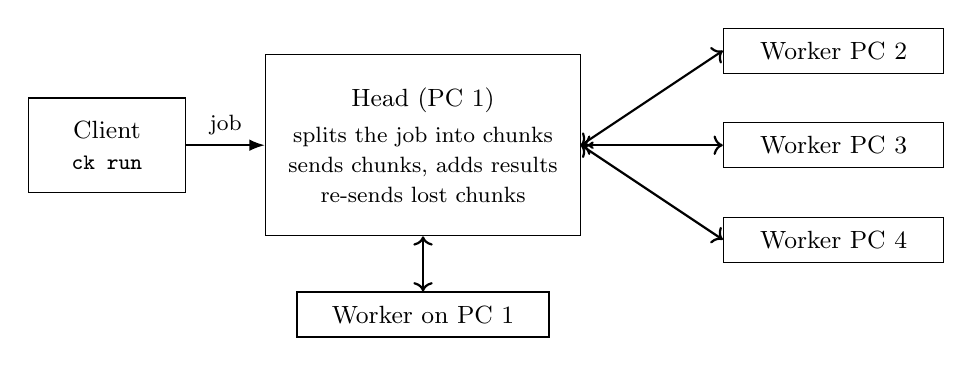
\begin{tikzpicture}[node distance=8mm and 12mm]
  \node[box,minimum width=2cm,minimum height=1.2cm] (cl) {Client\\\footnotesize\texttt{ck run}};
  \node[box,right=10mm of cl,minimum width=4cm,minimum height=2.3cm] (hd)
    {Head (PC 1)\\[2pt]\footnotesize splits the job into chunks\\\footnotesize sends chunks, adds results\\\footnotesize re-sends lost chunks};
  \node[box,right=18mm of hd,yshift=12mm,minimum width=2.8cm] (w2) {Worker PC 2};
  \node[box,right=18mm of hd,minimum width=2.8cm] (w3) {Worker PC 3};
  \node[box,right=18mm of hd,yshift=-12mm,minimum width=2.8cm] (w4) {Worker PC 4};
  \node[box,below=7mm of hd,minimum width=3.2cm] (lw) {Worker on PC 1};
  \draw[arr] (cl) -- node[above,font=\footnotesize]{job} (hd);
  \foreach \w in {w2,w3,w4} \draw[arr,<->] (hd.east) -- (\w.west);
  \draw[arr,<->] (hd) -- (lw);
\end{tikzpicture}
\caption{The head splits the job and shares it between three worker PCs and a worker running on the head PC itself.}
\label{fig:arch}
\end{figure}

When a job starts, the head cuts the range of numbers into chunks. Instead of dividing the work up front, it lets each worker ask for a chunk whenever it is free. A worker always keeps one extra chunk queued, so while it computes one chunk the next is already waiting and it never sits idle waiting for the network. A side effect is that faster PCs simply ask more often and end up doing more of the work, with no tuning on our part. Inside each PC the chunk is split again across all CPU cores using the Rayon library.

If a worker is unplugged or crashes in the middle of a job, the head notices the closed connection and gives that worker's unfinished chunks to the others, so the job still finishes. The head also serves a small web dashboard that shows each worker, its CPU use and the chunks it has completed.

\subsection{Networking}
We use two protocols for two different jobs (Table~\ref{tab:net}). To find each other, the head sends a small UDP broadcast every few moments saying \enquote{I am the head}. A worker started anywhere on the same network hears it and connects, so nobody has to type IP addresses. If one broadcast is lost it does not matter, because the next one follows shortly. The actual work and results travel over TCP instead, because every chunk and every result must arrive and nothing can be lost. Each worker keeps one TCP connection open for the whole job.

\begin{table}[H]\centering
\caption{Network ports used by Cluster Kit}\label{tab:net}
\begin{tabular}{lll}
\toprule
Protocol & Port & Purpose\\
\midrule
UDP & 7701 & head announces itself (discovery)\\
TCP & 7700 & chunks of work and results\\
HTTP & 7702 & live dashboard in a browser\\
\bottomrule
\end{tabular}
\end{table}

Figure~\ref{fig:seq} shows the messages exchanged between the head and one worker during a job.

\begin{figure}[H]\centering
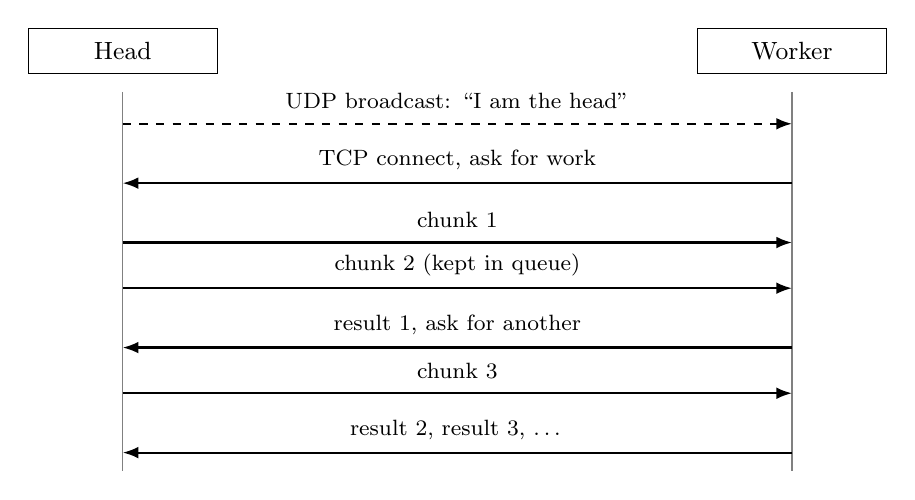
\begin{tikzpicture}[x=1cm,y=-0.58cm]
  \node[box,minimum width=2.4cm] at (0,0) {Head};
  \node[box,minimum width=2.4cm] at (8.5,0) {Worker};
  \draw[gray] (0,0.9) -- (0,9.2);
  \draw[gray] (8.5,0.9) -- (8.5,9.2);
  \newcommand{\msg}[4]{\ifx#3r\draw[arr,#4] (0,#1) -- (8.5,#1);\else\draw[arr,#4] (8.5,#1) -- (0,#1);\fi
    \node[font=\footnotesize,fill=white,inner sep=1pt] at (4.25,#1-0.5) {#2};}
  \msg{1.6}{UDP broadcast: \enquote{I am the head}}{r}{dashed}
  \msg{2.9}{TCP connect, ask for work}{l}{solid}
  \msg{4.2}{chunk 1}{r}{solid}
  \msg{5.2}{chunk 2 (kept in queue)}{r}{solid}
  \msg{6.5}{result 1, ask for another}{l}{solid}
  \msg{7.5}{chunk 3}{r}{solid}
  \msg{8.8}{result 2, result 3, \dots}{l}{solid}
\end{tikzpicture}
\caption{Messages between the head and one worker. The dashed arrow is UDP; the rest go over one TCP connection.}
\label{fig:seq}
\end{figure}

\subsection{Other parts of the project}
Jobs do not have to be written in Rust. Our test program, \texttt{simple\_sha256.py}, is plain Python, and the engine can run it on every worker; the head can even send the script to workers that do not have a copy, so no shared folder is needed. The repository also contains a second engine based on Dask~\cite{dask} for Python users. The engine itself is one portable program that runs on Ubuntu, Windows and macOS.

\section{Test setup}
We ran all tests in our lab on four identical desktops running Ubuntu 26.04.1, each with 12 CPU threads and 7.1\,GB of RAM, connected by wired Ethernet (round-trip time under 1\,ms). We labelled the head PC \enquote{Master} with a sticky note so we would not mix them up (Figure~\ref{fig:lab}). We built \texttt{ck} once on the head and copied the program to the three workers.

\begin{figure}[H]\centering
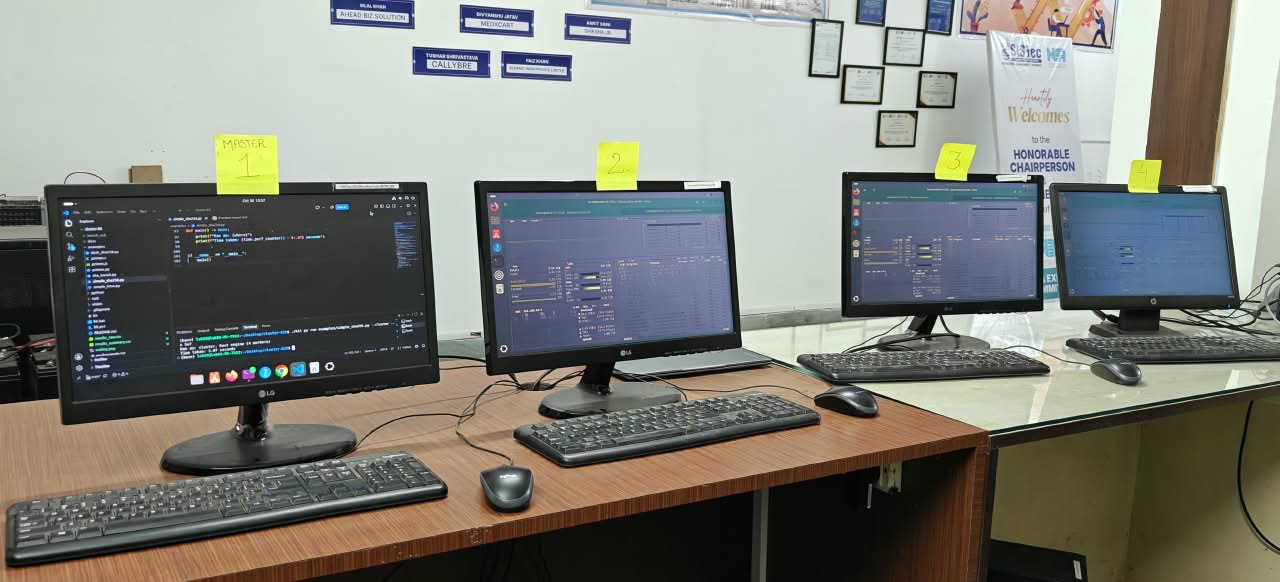
\includegraphics[width=0.6\textwidth]{img/testbed.jpg}
\caption{The four PCs we used. PC 1, marked \enquote{Master}, is the head.}
\label{fig:lab}
\end{figure}

For the scaling test (Section~\ref{sec:ctl}) we measured seven setups: each PC on its own, then 2, 3 and 4 PCs. To keep the comparison fair we ran every setup seven times, rotating through the setups after one warm-up run, so that any slow drift such as the PCs heating up would affect all of them equally. We report the median of the seven runs.

\section{Results}\label{sec:results}
\subsection{Windows laptop and the cluster}
Before the controlled test we ran our Python example on a normal Windows laptop and then on the four-PC cluster. Both runs found the same 766 matching hashes, so they did exactly the same work. The laptop took 36.98 seconds and the cluster took 2.165 seconds, 17 times faster (Figure~\ref{fig:laptop}, Table~\ref{tab:laptop}).

\begin{figure}[H]\centering
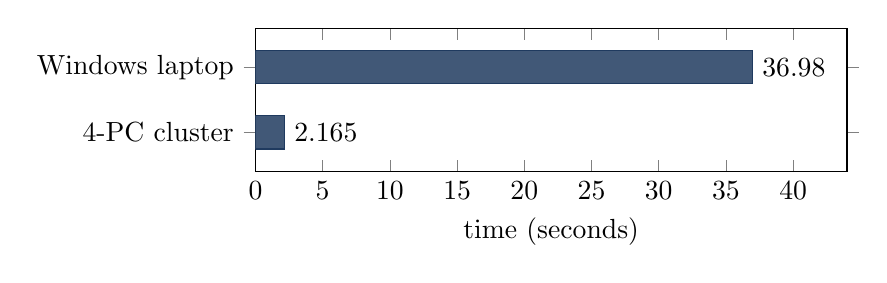
\begin{tikzpicture}
\begin{axis}[xbar,width=0.75\textwidth,height=3.4cm,bar width=12pt,xmin=0,xmax=44,
  ytick={1,2},yticklabels={4-PC cluster,Windows laptop},enlarge y limits=0.6,
  xlabel={time (seconds)},nodes near coords,nodes near coords align={horizontal},/pgf/number format/precision=3]
\addplot[fill=gblue!85,draw=gblue] coordinates {(2.165,1) (36.98,2)};
\end{axis}
\end{tikzpicture}
\caption{Time taken by the same program on a Windows laptop and on the cluster.}
\label{fig:laptop}
\end{figure}

\begin{table}[H]\centering
\caption{Windows laptop compared with the cluster}\label{tab:laptop}
\begin{tabular}{lrrr}
\toprule
 & Windows laptop & 4-PC cluster & Difference\\
\midrule
Time & 36.98 s & 2.165 s & 34.815 s saved\\
Matching hashes & 766 & 766 & same\\
Speed-up & 1 & 17.08 & 94.1\% less time\\
\bottomrule
\end{tabular}
\end{table}

This number needs some care. The laptop is a different machine, the run was done only once, and we did not record whether it used one core or all of them, while the cluster had 48 threads. So the 17 times figure shows the practical gain over a laptop, not what clustering alone adds. For that we did the controlled test below. During our live demo in the lab the cluster ran the same program on 50 million numbers in 3.87 seconds (Figure~\ref{fig:live}).

\subsection{Controlled scaling test}\label{sec:ctl}
Here we kept everything the same (the PCs, the program and the amount of work per PC) and changed only the number of PCs. Table~\ref{tab:scale} and Figure~\ref{fig:scale} show the results.

\begin{table}[H]\centering
\caption{Scaling results, median of seven runs}\label{tab:scale}
\begin{tabular}{crrrr}
\toprule
PCs & M hashes/s & Speed-up & Efficiency & Time for $10^{11}$ hashes\\
\midrule
1 & 20.55 & 0.91 & 100.0\% & 81 min\\
2 & 44.86 & 1.98 & 102.1\% & 37 min\\
3 & 67.48 & 2.98 & 100.3\% & 25 min\\
4 & 87.38 & 3.86 & 96.4\% & 19 min\\
\bottomrule
\end{tabular}
\end{table}

\begin{figure}[H]\centering
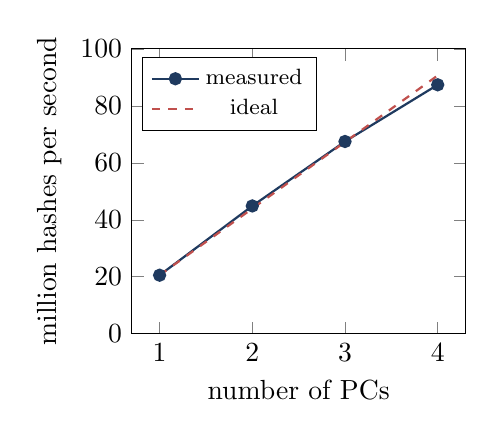
\begin{tikzpicture}
\begin{axis}[width=0.48\textwidth,height=5.2cm,xlabel={number of PCs},ylabel={million hashes per second},
  xtick={1,2,3,4},ymin=0,ymax=100,legend pos=north west,legend style={font=\footnotesize}]
\addplot[gblue,thick,mark=*] coordinates {(1,20.55)(2,44.86)(3,67.48)(4,87.38)};
\addplot[accent,thick,dashed] coordinates {(1,20.55)(2,43.93)(3,67.30)(4,90.65)};
\legend{measured,ideal}
\end{axis}
\end{tikzpicture}\hfill
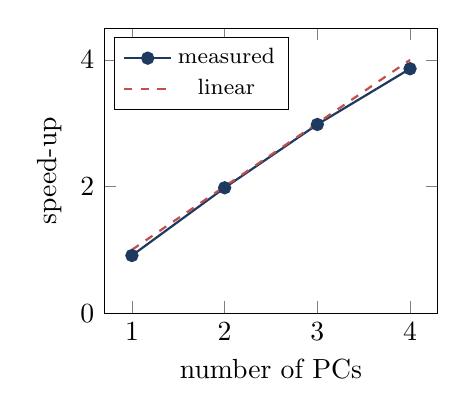
\begin{tikzpicture}
\begin{axis}[width=0.48\textwidth,height=5.2cm,xlabel={number of PCs},ylabel={speed-up},
  xtick={1,2,3,4},ymin=0,ymax=4.5,legend pos=north west,legend style={font=\footnotesize}]
\addplot[gblue,thick,mark=*] coordinates {(1,0.91)(2,1.98)(3,2.98)(4,3.86)};
\addplot[accent,thick,dashed,domain=1:4] {x};
\legend{measured,linear}
\end{axis}
\end{tikzpicture}
\caption{Left: hashing speed against the ideal, which is the sum of each PC's own speed. Right: speed-up against perfect linear scaling.}
\label{fig:scale}
\end{figure}

With all four PCs the cluster hashed 87.38 million numbers per second, 3.86 times the speed of an average single PC and 96.4\% of what the four PCs manage separately. Less than 4\% of the time went into coordination. In practical terms, a job that would take 81 minutes on one of our lab PCs takes about 19 minutes on four. Each added PC gave a clear, statistically significant improvement (permutation test, $p = 0.0003$), and every repeated run returned the same number of matches.

We noticed one oddity. On its own, PC 1 was about 12\% slower than the other three, even though the machines are identical. It was the head and was also running another of our services at the time, which most likely took some of its CPU. Because of this we calculate the speed-up against the average single PC (22.66 million hashes per second) rather than against PC 1 alone, which would have inflated the result to 4.25.

\begin{figure}[H]\centering
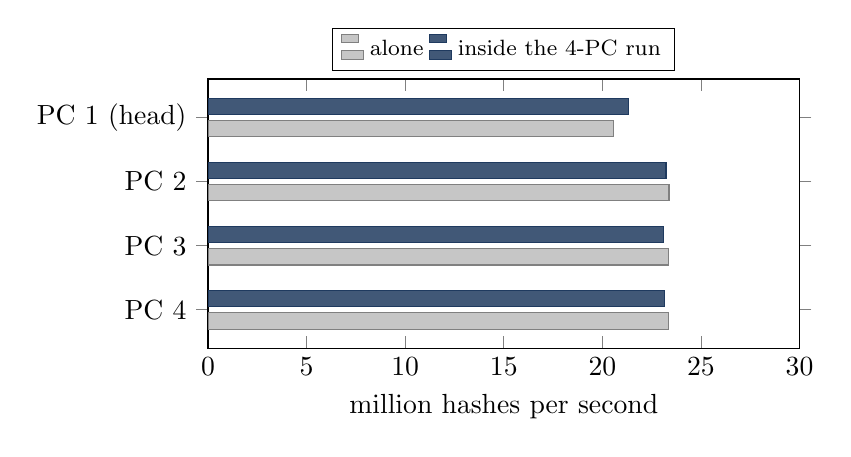
\begin{tikzpicture}
\begin{axis}[xbar,width=0.75\textwidth,height=5cm,bar width=6pt,xmin=0,xmax=30,
  ytick={1,2,3,4},yticklabels={PC 4,PC 3,PC 2,PC 1 (head)},enlarge y limits=0.2,
  xlabel={million hashes per second},legend style={at={(0.5,1.03)},anchor=south,font=\footnotesize},legend columns=2]
\addplot[fill=gray!45,draw=gray] coordinates {(23.35,1)(23.37,2)(23.38,3)(20.55,4)};
\addplot[fill=gblue!85,draw=gblue] coordinates {(23.15,1)(23.12,2)(23.23,3)(21.31,4)};
\legend{alone,inside the 4-PC run}
\end{axis}
\end{tikzpicture}
\caption{Each PC's speed on its own and while working inside the four-PC cluster.}
\label{fig:perpc}
\end{figure}

Figure~\ref{fig:perpc} shows that each PC kept almost all of its own speed while working in the cluster. The work also split nearly evenly, with each PC doing between 23.9\% and 25.7\% of the numbers, even though we never told the head how to divide it. PC 1 did the smallest share, which fits with it being the slowest. Every PC spent 96--99\% of the job actually computing.

\begin{figure}[H]\centering
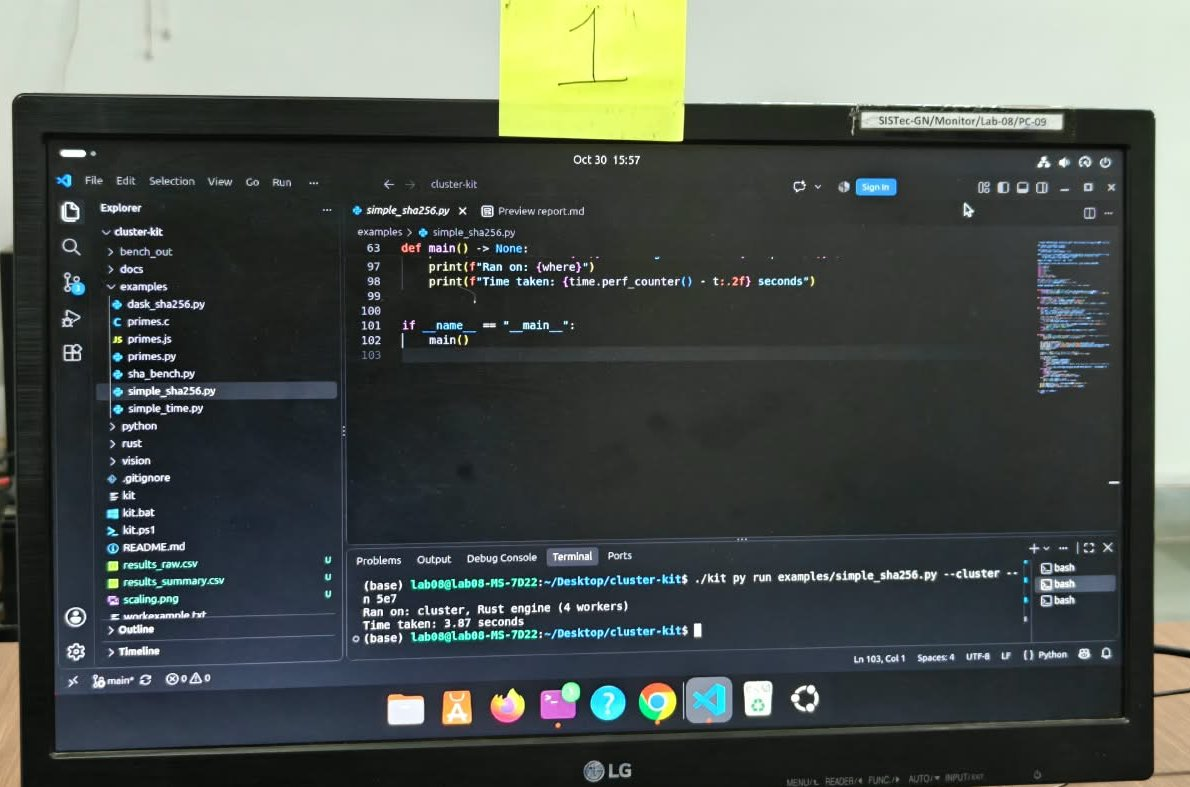
\includegraphics[height=4.2cm]{img/terminal.jpg}\hfill
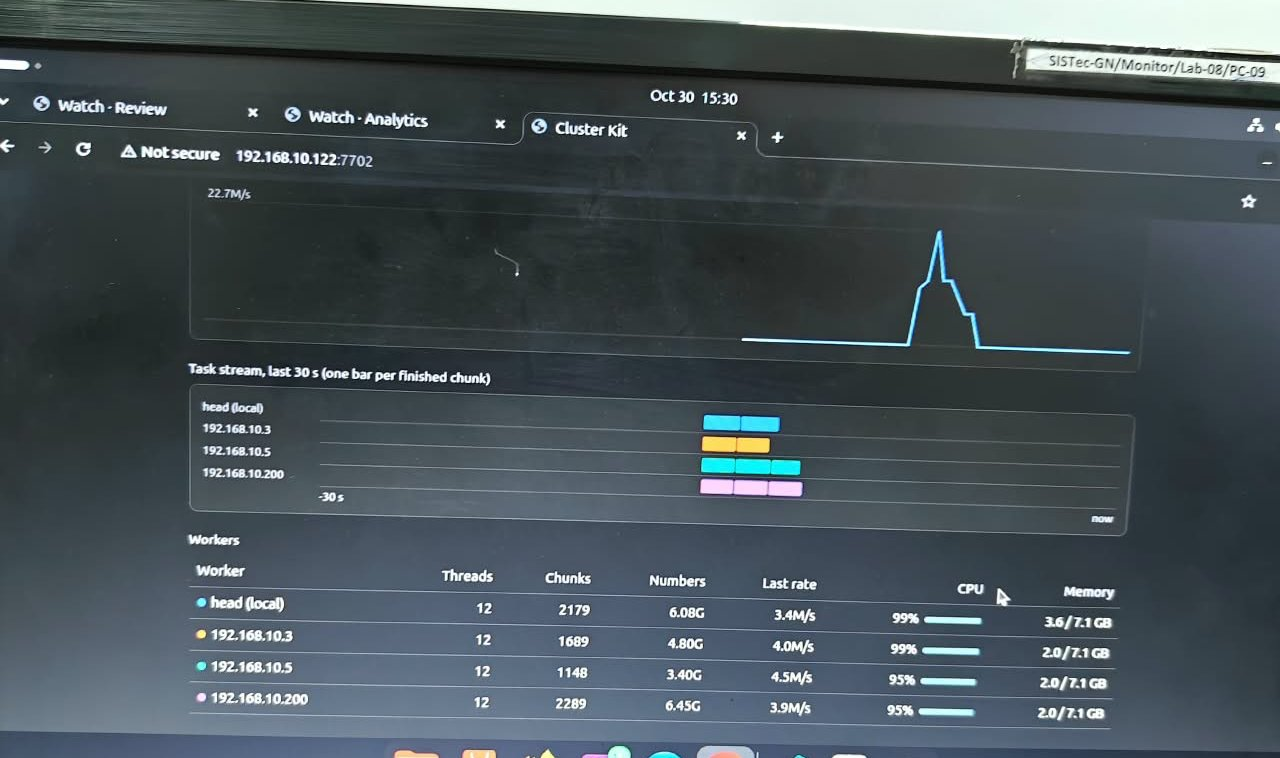
\includegraphics[height=4.2cm]{img/dashboard.jpg}
\caption{From our lab demo. Left: the head PC after running \texttt{simple\_sha256.py} on the cluster (\enquote{Ran on: cluster, Rust engine (4 workers)}, 3.87\,s). Right: the dashboard during a run, with all four PCs at 95--99\% CPU.}
\label{fig:live}
\end{figure}

\section{Comparison with MPI}\label{sec:mpi}
Real supercomputers mostly use MPI~\cite{mpi}, the Message Passing Interface. MPI is built for the highest possible speed on dedicated hardware and supports any pattern of communication between processes. Cluster Kit aims at something different: the least possible setup on ordinary lab PCs. We did not benchmark MPI ourselves, so Table~\ref{tab:mpi} compares only how the two are set up and how they behave.

\begin{table}[H]\centering
\caption{Cluster Kit and a typical MPI setup}\label{tab:mpi}
\begin{tabularx}{\textwidth}{lLL}
\toprule
 & Typical MPI setup & Cluster Kit\\
\midrule
Finding the PCs & IP addresses listed in a host file & automatic, using UDP broadcast\\
Starting a job & SSH keys and \texttt{mpirun} on every PC & start the program on each PC\\
Dividing the work & usually fixed in advance & each PC asks for work when it is free\\
PCs of different speed & the slowest one sets the pace & faster PCs do more\\
If a PC fails & the job usually stops & its chunks go to the other PCs\\
Communication & any pattern between processes & only independent chunks\\
\bottomrule
\end{tabularx}
\end{table}

For our kind of job, where every chunk is independent, we expect MPI would be about as fast, since there is less than 4\% left to gain. Where Cluster Kit is clearly easier is the setup and the way it copes with a PC dropping out. Measuring an MPI version on the same four PCs would be a good next step.

\section{Limitations and future work}
Cluster Kit only helps with work that can be cut into independent pieces; programs whose parts need to talk to each other constantly would need something like MPI. All PCs also have to be on the same local network, and the head PC coordinates every job, so if the head goes down the job stops. Our tests used only four PCs and short runs of about three seconds each.

There are several things we would like to try next: running on more than four PCs to see where the head becomes a bottleneck, adding GPU workers, adding authentication and encryption, measuring an MPI version for a direct comparison, and running real scientific or data-processing jobs instead of a hash search.

\section{Conclusion}
We set out to see whether the lab PCs we use every day could work together like a small supercomputer. With Cluster Kit, four of them ran our test job 3.86 times faster than one PC, at 96.4\% efficiency, and the same program finished 17 times faster than on a Windows laptop. The PCs find each other on their own, the work spreads evenly without any tuning, and the job survives a PC dropping out. The same method should carry over to a whole lab, and to the 500 computers a college may have, which is the next thing we want to measure. For work that splits into independent pieces, a handful of ordinary desktops gets surprisingly close to the ideal.

{\footnotesize\setlength{\itemsep}{0pt}\setlength{\parskip}{1pt}
\begin{thebibliography}{9}
\bibitem{amdahl} G.~M. Amdahl, \enquote{Validity of the single processor approach to achieving large scale computing capabilities,} in \emph{Proc. AFIPS Spring Joint Computer Conference}, 1967, pp.~483--485.
\bibitem{gustafson} J.~L. Gustafson, \enquote{Reevaluating Amdahl's law,} \emph{Communications of the ACM}, vol.~31, no.~5, pp.~532--533, 1988.
\bibitem{mpi} Message Passing Interface Forum, \emph{MPI: A Message-Passing Interface Standard, Version 4.0}, 2021.
\bibitem{dask} M.~Rocklin, \enquote{Dask: Parallel computation with blocked algorithms and task scheduling,} in \emph{Proc. 14th Python in Science Conference}, 2015, pp.~130--136.
\bibitem{fips} National Institute of Standards and Technology, \enquote{Secure Hash Standard (SHS),} FIPS PUB 180-4, 2015.
\bibitem{repo} Cluster Kit source code, \url{https://github.com/TheDivyanshShukla/cluster-kit}.
\end{thebibliography}}

\end{document}
